\section{Übung - OLAP}
\label{sec:uebung_06}

% ##########################################################################
% ############################### Aufgabe 01 ###############################
% ##########################################################################
\label{subsec:uebung_06.aufgabe_01}
\subsection{Aufgabe}
Erzeuge folgende Übersicht über die Anzahl der Mitarbeiter in jeder Abteilung, in jeder Stadt und in jedem Land.

\begin{figure}[H]
  \centering
  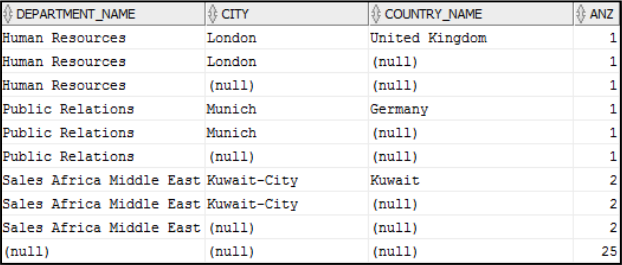
\includegraphics[width=1\textwidth]{img//uebung_06_-_aufgabe_01.png}
  \label{img:uebung_06_-_aufgabe_01}
\end{figure} 

\subsubsection*{Lösung}
\label{subsubsec:uebung_06.aufgabe_01.loesung}
\inputsql{./sql/uebung_06/uebung_06_-_aufgabe_01.sql}


% ##########################################################################
% ############################### Aufgabe 02 ###############################
% ##########################################################################
\label{subsec:uebung_06.aufgabe_02}
\subsection{Aufgabe}
Erzeuge folgende Übersicht über die Anzahl der Mitarbeiter in jeder Abteilung, in jeder Stadt und in jedem Land.

\begin{WARN}
 Tabelle fehlt!
\end{WARN}

\subsubsection*{Lösung}
\label{subsubsec:uebung_06.aufgabe_02.loesung}
\inputsql{./sql/uebung_06/uebung_06_-_aufgabe_02.sql}


% ##########################################################################
% ############################### Aufgabe 03 ###############################
% ##########################################################################
\label{subsec:uebung_06.aufgabe_03}
\subsection{Aufgabe}
Die Vertriebsabteilung benötigt eine Auswertung über den Umsatz zwischen 2010 und 2012 insgesamt, je Jahr, je Land und Region sowie je Jahr, Land und Region.

\begin{WARN}
 Tabelle fehlt!
\end{WARN}

\subsubsection*{Lösung}
\label{subsubsec:uebung_06.aufgabe_03.loesung}
\inputsql{./sql/uebung_06/uebung_06_-_aufgabe_03.sql}


% ##########################################################################
% ############################### Aufgabe 04 ###############################
% ##########################################################################
\label{subsec:uebung_06.aufgabe_04}
\subsection{Aufgabe}
Geben Sie für jeden Job, die Anzahl der Mitarbeiter in den Ländern 'United Kingdom', 'United States of America', 'Germany', 'Kuwait', 'Canada' und 'Singapore' in einer Zeile aus.

\begin{figure}[H]
  \centering
  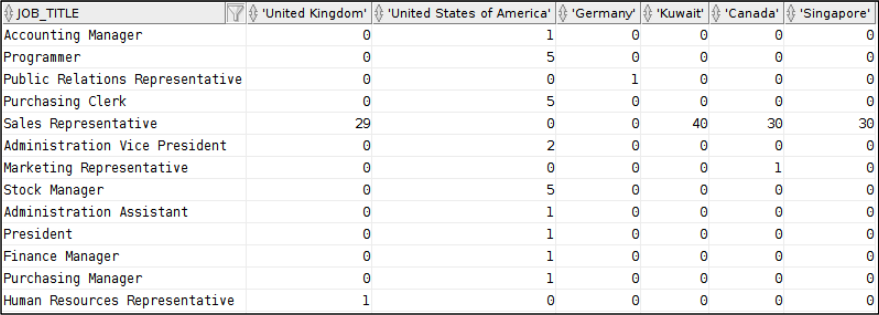
\includegraphics[width=1\textwidth]{img//uebung_06_-_aufgabe_04.png}
  \label{img:uebung_06_-_aufgabe_04}
\end{figure} 

\subsubsection*{Lösung}
\label{subsubsec:uebung_06.aufgabe_04.loesung}
\inputsql{./sql/uebung_06/uebung_06_-_aufgabe_04.sql}

